\section{Numerical study}\label{sec:blup:numerical_study}

\color{magenta}
In this section, we present a finite-sample Monte Carlo simulation study and a real data application. The simulation study is based on national electricity consumption curves for France, available from the ODR\'E platform \citep{odre_data}. These curves are used to estimate the parameters of a first-order autoregressive process (FAR(1)), which are then used to generate synthetic curves for the Monte Carlo simulations. \color{black}For the real data application, we analyse \color{magenta}[TBC: two applications replace the Facebook study, NOTPERP intraday log-return curves in the random design and French electricity curves in the common design; provenance from 41--43\_notperp\_*.R and 40\_app\_energy.R]\color{black}. \color{magenta}All results were obtained using the \texttt{R} package \texttt{adaptiveFTS} and supplementary code, both of which are publicly available at \url{https://github.com/hmaissoro}. An Epanechnikov kernel ($K(u) = (3/4)(1 - u^2)$ for $|u| \leq 1$, and $0$ otherwise) is used in all experiments.
\color{black}

\subsection{\color{magenta}Simulation design\color{black}}\label{blup:sec:simu_exp}
The Monte Carlo simulation is based on France's daily national electricity consumption curves from June to September 2024. The dataset contains 122 curves, one for each day within this period. Each curve represents electricity consumption recorded at 96 evenly spaced time points throughout the day, with measurements taken every 15 minutes. For readability, we normalise the curves to the interval $[0,1]$ by dividing each value by the maximum consumption observed over the entire period. Figure~\ref{fig:conso_last_curves} displays the last \color{magenta}three\color{black} consumption curves from the dataset.

\color{magenta}
To simulate FTS with patterns similar to those of the observed curves, we estimate the parameters of a FAR(1) model from the data and use them to generate synthetic FTS samples. We consider the FAR(1) process with an associated innovation process $\{\xi_n\}$, defined as:
\color{black}
\begin{equation}\label{blup:FTS_mod1}
	\color{magenta}X_n(u) = \mu(u) + \int_0^1\psi(u,s)(X_{n-1}(s)-\mu(s))\,ds + L_t\xi_n(u),\color{black}
\end{equation}
\color{magenta}
where the mean function $\mu$ and the kernel of the autoregressive operator $\psi$ are estimated from the real consumption curves. The innovation process $\{\xi_n\}$ is independently generated as a multi-fractional Brownian motion, with the Hurst index function also estimated from the real consumption curves \citep[see][]{taqqu2006}. Let us note that, as shown in Example 2 of \citet{Maissoro2025}, if the kernel $\psi(\cdot,s)$ is Hölder continuous with a Hölder exponent greater than the regularity of $\{\xi_n\}$, then the FTS $\{X_n\}$ inherits the regularity of the innovation process. In particular, $\{X_n\}$ has a local Hölder exponent corresponding to the Hurst index function of $\{\xi_n\}$ and a Hölder constant $L_t^2$.
[TBC: notation superseded, needs review. $\psi$ denotes the solution of $C_1 = \psi C_0$ in best\_predictor\_aout24.tex, not a kernel; $L_t$ is not attested there, and 11\_simulation\_generate.R passes \texttt{L2 = 0.01} to the covariance, so the constant is $\sqrt{\texttt{L2}}$; the display omits the per-curve random intercept \texttt{intercept\_var = 0.05}; and the Hurst function is \texttt{hurst\_linear(h\_left = 0.4, h\_right = 0.8)}, an analytic ramp, not an estimate from the consumption curves]\color{black}

\color{magenta}
[TBC: the paragraph describing estimation of the local Hölder exponent from the real dataset is invalidated by the analytic Hurst ramp in 11\_simulation\_generate.R:57; the Fourier estimation of $\mu$ and $\psi$ survives and should be restated from 02\_energy\_conso.R]
\color{black}

\begin{figure}[t!]
	\centering
	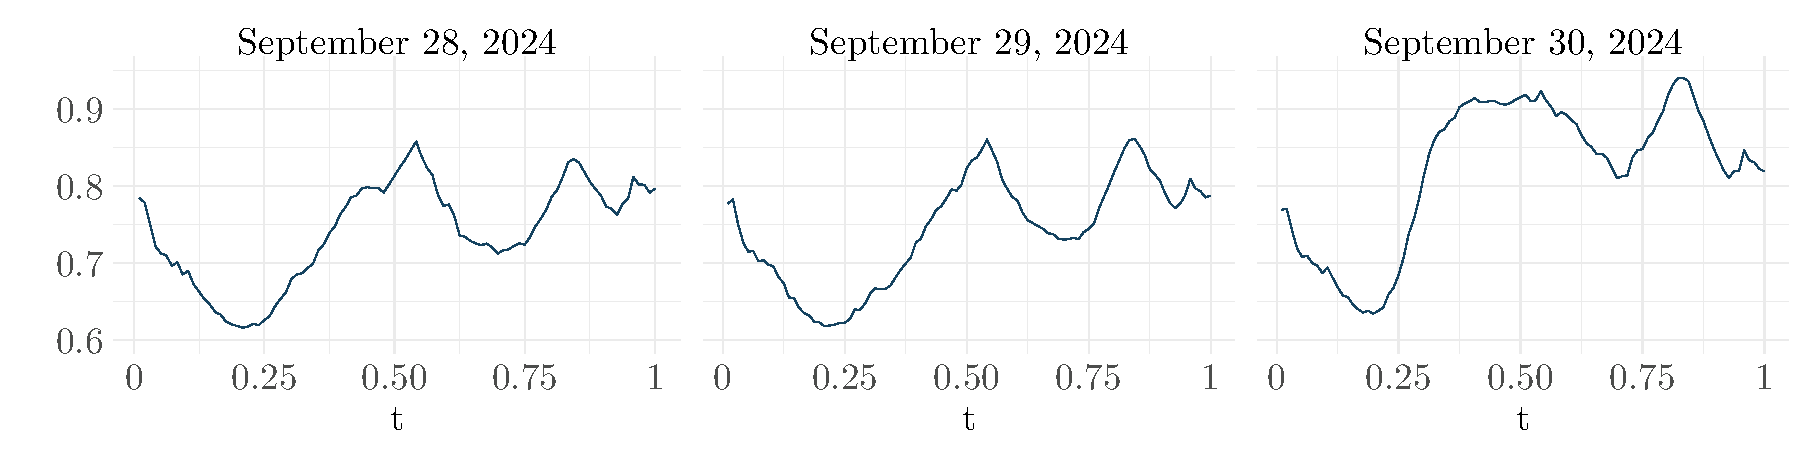
\includegraphics[width=\textwidth]{./figures/real_data_conso_3last_curves.pdf}
	\caption{\small The last \color{magenta}three\color{black} daily national electricity consumption curves in France from the dataset, with values normalised to the interval $[0,1]$.}
	\label{fig:conso_last_curves}
\end{figure}

\begin{figure}[h!]
	\centering
	\begin{tabular}{ccc}
		\small (a) $\footnotesize \widehat{H}_t$ for simulation & \small (b) $\footnotesize \widehat{\mu}$ for simulation & \small (c) $\footnotesize \widehat{\psi}$ for simulation\\
		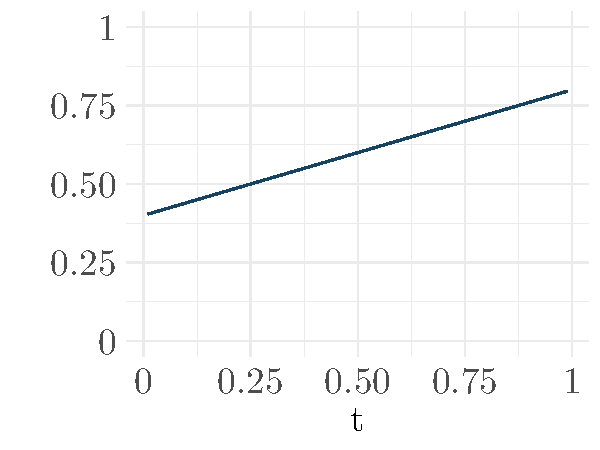
\includegraphics[width=0.3\textwidth]{./figures/local_exponent_simulation_conso.pdf} & 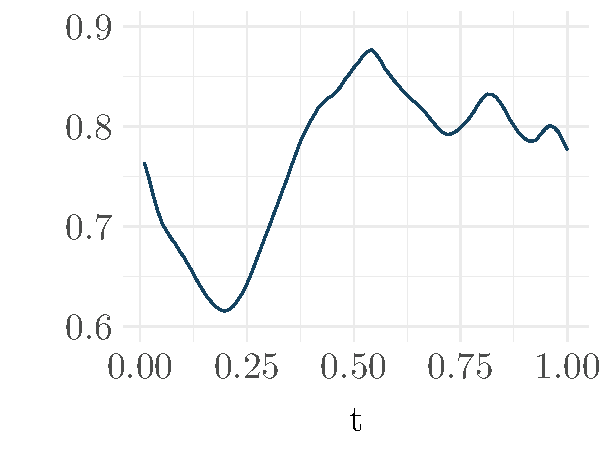
\includegraphics[width=0.3\textwidth]{./figures/smooth_mean_conso.pdf} &
		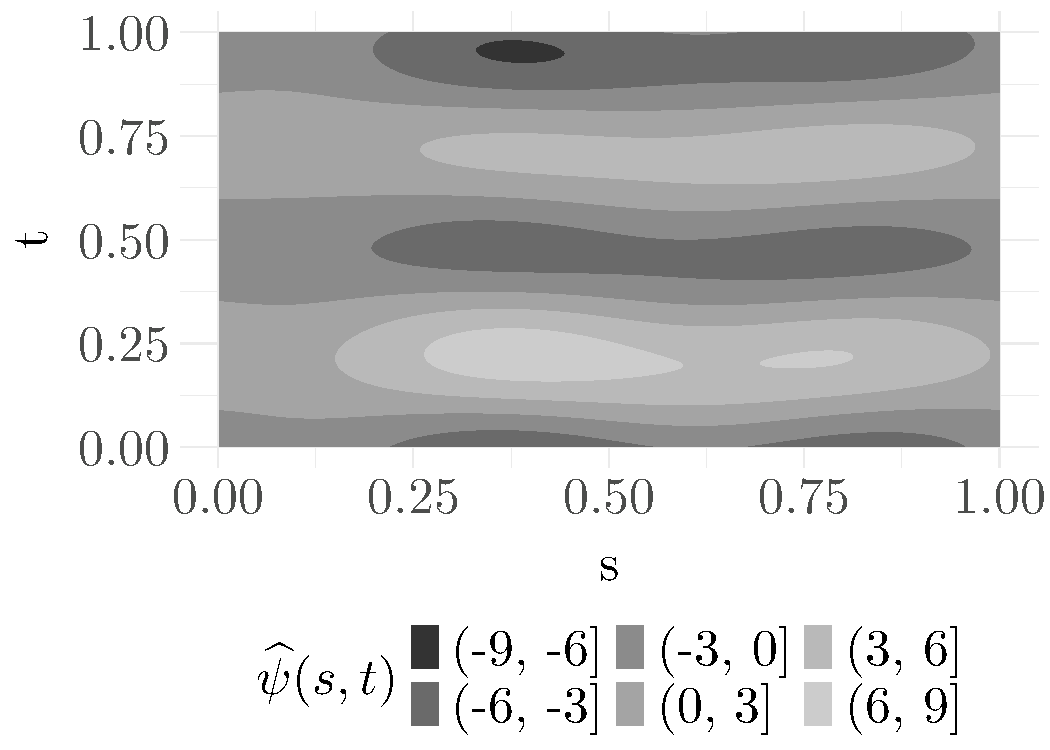
\includegraphics[width=0.3\textwidth]{./figures/far_kernel_conso.pdf}
	\end{tabular}
	\caption{\small Simulation parameters estimated from consumption curves: (a) estimated local exponent function, (b) estimated mean function, (c) estimated autoregressive kernel. \color{magenta}[TBC: panel (a) is not an estimate. 10\_simulation\_design.R:200 and 219--231 plot \texttt{get\_local\_exponent}, the analytic ramp \texttt{hurst\_linear(h\_left = 0.4, h\_right = 0.8)} itself, so the column header $\widehat{H}_t$, the word ``estimated'' in this caption and the blanket ``estimated from consumption curves'' are all wrong for (a). Panels (b) and (c) are estimates and the caption holds for them: 02\_energy\_conso.R:138 plots \texttt{get\_conso\_mean} and :382 plots \texttt{get\_far\_kenel\_conso} at \texttt{operator\_norm = 0.5}, both of which the simulator then uses. Decide whether (a) keeps the hat, and whether the estimated local regularity of the data --- \texttt{plot\_locreg\_conso\_data}, 10\_simulation\_design.R:193 --- belongs here instead or alongside]\color{black}}
	\label{fig:simu_param}
\end{figure}

\color{magenta}
To obtain the data points according to \eqref{eq:model}, the number of points on each curve, $M_n$, is randomly generated from a uniform distribution between $0.8\lambda$ and $1.2\lambda$, while the observation times $\{T_{n,i}\}$ are drawn independently from a uniform distribution on the interval $(0,1]$. We set $L_t = 0.1$, corresponding to the mean of the estimates of the local Hölder constant of the consumption curves, evaluated over an equidistant grid of $99$ points between $0.01$ and $0.99$, and obtained using the estimator proposed by \citet{Maissoro2025}. For the observation error term, we set $\sigma(T_{n,i}) = 0.007$, corresponding to the mean standard deviation of the consumption curves estimated using [TBC: \texttt{eq:blup:sigma\_estimator} --- label not defined in best\_predictor\_aout24.tex] over the observation grid, and the $\varepsilon_{n,i}$ are centred Gaussian variables with unit variance. A sequence of $100$ burn-in steps is used to initialise \eqref{blup:FTS_mod1}. Figure~\ref{fig:generated_last_curves} illustrates the simulated sample paths and the randomly observed points for a sample size of $(N, \lambda) = (150, 25)$.
[TBC: notation superseded, needs review. $L_t = 0.1$ is consistent with \texttt{L2 = 0.01} but the provenance sentence is invalidated by the analytic Hurst ramp; the per-curve intercept and the fact that each sample carries both designs are unstated]\color{black}

\color{magenta}
[TBC: the paragraph stating that the BLUP study generates a single sample and regenerates its last curve is invalidated. 11\_simulation\_generate.R draws a new FAR series per replication: 400 replications for each of the twelve configurations $(N,\lambda) \in \{150,300,600\}\times\{25,50,100,200\}$, seeded by $N\cdot 10^6 + \lambda\cdot 10^3 + \texttt{id\_mc}$, with 100 burn-in curves discarded and both designs carried on the same curves]
\color{black}

\subsection{\color{magenta}(Auto)covariance function estimation\color{black}}\label{sec:emp_study:autocov}

\color{magenta}
We conclude this section with a performance comparison of the new autocovariance estimator against the \texttt{MPV25} estimator, which uses a single bandwidth. Let $\widehat{c}_{N,\ell}^{(i)}$ denote our new estimator computed from the $i$-th replication ($i = 1, \ldots, R = 400$), and let $\widehat{c}_{\texttt{MPV25}, \ell}^{(i)}$ denote the corresponding \texttt{MPV25} estimator. For benchmarking, we use the empirical infeasible estimator, denoted by ${\widehat{c}}_{N', \ell}$, which is computed on a large sample of size $N'$. This estimator is feasible in simulation settings. That is,
\color{black}
\begin{equation}
	\color{magenta}\widehat{c}_{N', \ell}(s, t) = \frac{1}{N' - \ell} \sum_{n=1}^{N' - \ell} \left\{X_{n}(s) - \widehat{\mu}_{N'}(s)\right\} \left\{X_{n+\ell}(t) - \widehat{\mu}_{N'}(t)\right\},
	\qquad \text{where} \quad
	\widehat{\mu}_{N'}(t) = \frac{1}{N'} \sum_{n=1}^{N'} X_n(t).\color{black}
\end{equation}
\color{magenta}
Then, for each $i = 1, \ldots, R$, we compute the pointwise error ratio:
\color{black}
\begin{equation}\label{eq:error_ratio_autocov}
	\color{magenta}\forall (s, t) \in I^2, \quad
	E_\ell^{(i)}(s, t) = \frac{\left| \widehat{c}_{N,\ell}^{(i)}(s, t; h_\ell^*(s|t), h_\ell^*(t|s)) - \widehat{c}_{N',\ell}(s, t) \right|}{\left| \widehat{c}_{\texttt{MPV25}, \ell}^{(i)}(s, t; h^*) - \widehat{c}_{N',\ell}(s, t) \right|}.\color{black}
\end{equation}
\color{magenta}
The benchmark is computed once, outside the Monte Carlo. A single series of $N' = 5000$ curves is generated from \eqref{blup:FTS_mod1} with the same parameters, on the equidistant grid of $99$ points between $0.01$ and $0.99$ common to every curve, and is retained without measurement error. It stands in for the unknown $c_\ell$, so that the two estimators are compared through their distance to it rather than to each other.
\color{black}

\color{magenta}
We report the comparison at four pairs $(s,t)$, chosen so that the distance between the two local exponents takes a different value at each of them. At $(0.7, 0.8)$ we have $(H_s, H_t) = (0.68, 0.72)$, at $(0.2, 0.4)$ we have $(0.48, 0.56)$, at $(0.4, 0.7)$ we have $(0.56, 0.68)$, and at $(0.8, 0.2)$ we have $(0.72, 0.48)$. The four values of $|H_s - H_t|$ are $0.04$, $0.08$, $0.12$ and $0.24$, one to each pair, and they are the distinct values the local exponent of Figure~\ref{fig:simu_param}-(a) produces over the pairs at which the estimators were computed. The theory leads us to expect the least gain from two bandwidths at the first pair and the most at the last.

Figure~\ref{fig:autocov_ratio_lag1} shows the boxplots of the error ratio \eqref{eq:error_ratio_autocov} at these four pairs, for each of the twelve setups $(N, \lambda)$. As expected the ratio lies below one at every pair in almost every setup: over the $48$ pairs of location and setup, its median is below one in $40$ of them, exactly one in $6$ and above one in $2$. The gain is largest at $(0.8, 0.2)$, where the two exponents are furthest apart; the median there runs from $0.433$ to $0.911$ and is the lowest of the four in eleven of the twelve setups.

The ordering does not carry through the middle of the range. At $(0.4, 0.7)$, whose gap is the larger of the two intermediate ones, the median ratio exceeds the median at $(0.2, 0.4)$ in eleven of the twelve setups. This is likely due to where the pair sits rather than to the size of its gap: both arguments of $(0.4, 0.7)$ lie on the smooth half of the domain and both call for a wide bandwidth, so one bandwidth serves them almost as well as two; $(0.8, 0.2)$ joins the smoothest of the four points to the roughest, and no single bandwidth serves both.

The medians equal to one have the same origin. The ratio is exactly one whenever the adaptive rule selects the same bandwidth for the two arguments, which it does in none of the $4800$ replications at $(0.8, 0.2)$, against between $5$ and $41$ of the $400$ replications of a setup at $(0.7, 0.8)$ --- the most of the four pairs in eleven of the twelve setups. As a consequence the four pairs differ not only in the size of the gain but in how often there is any gain to be had.

Two features of the display are declared rather than left to be inferred. The estimator returns no value in $532$ of the $19200$ combinations of replication, location and setup, and those replications are absent from the boxes. The vertical axis stops at $1.5$, and $5456$ of the remaining $18668$ ratios lie at or above it, so the boxes describe the lower part of the distribution and not the whole of it.
\color{black}

\begin{figure}[h!]
	\centering
	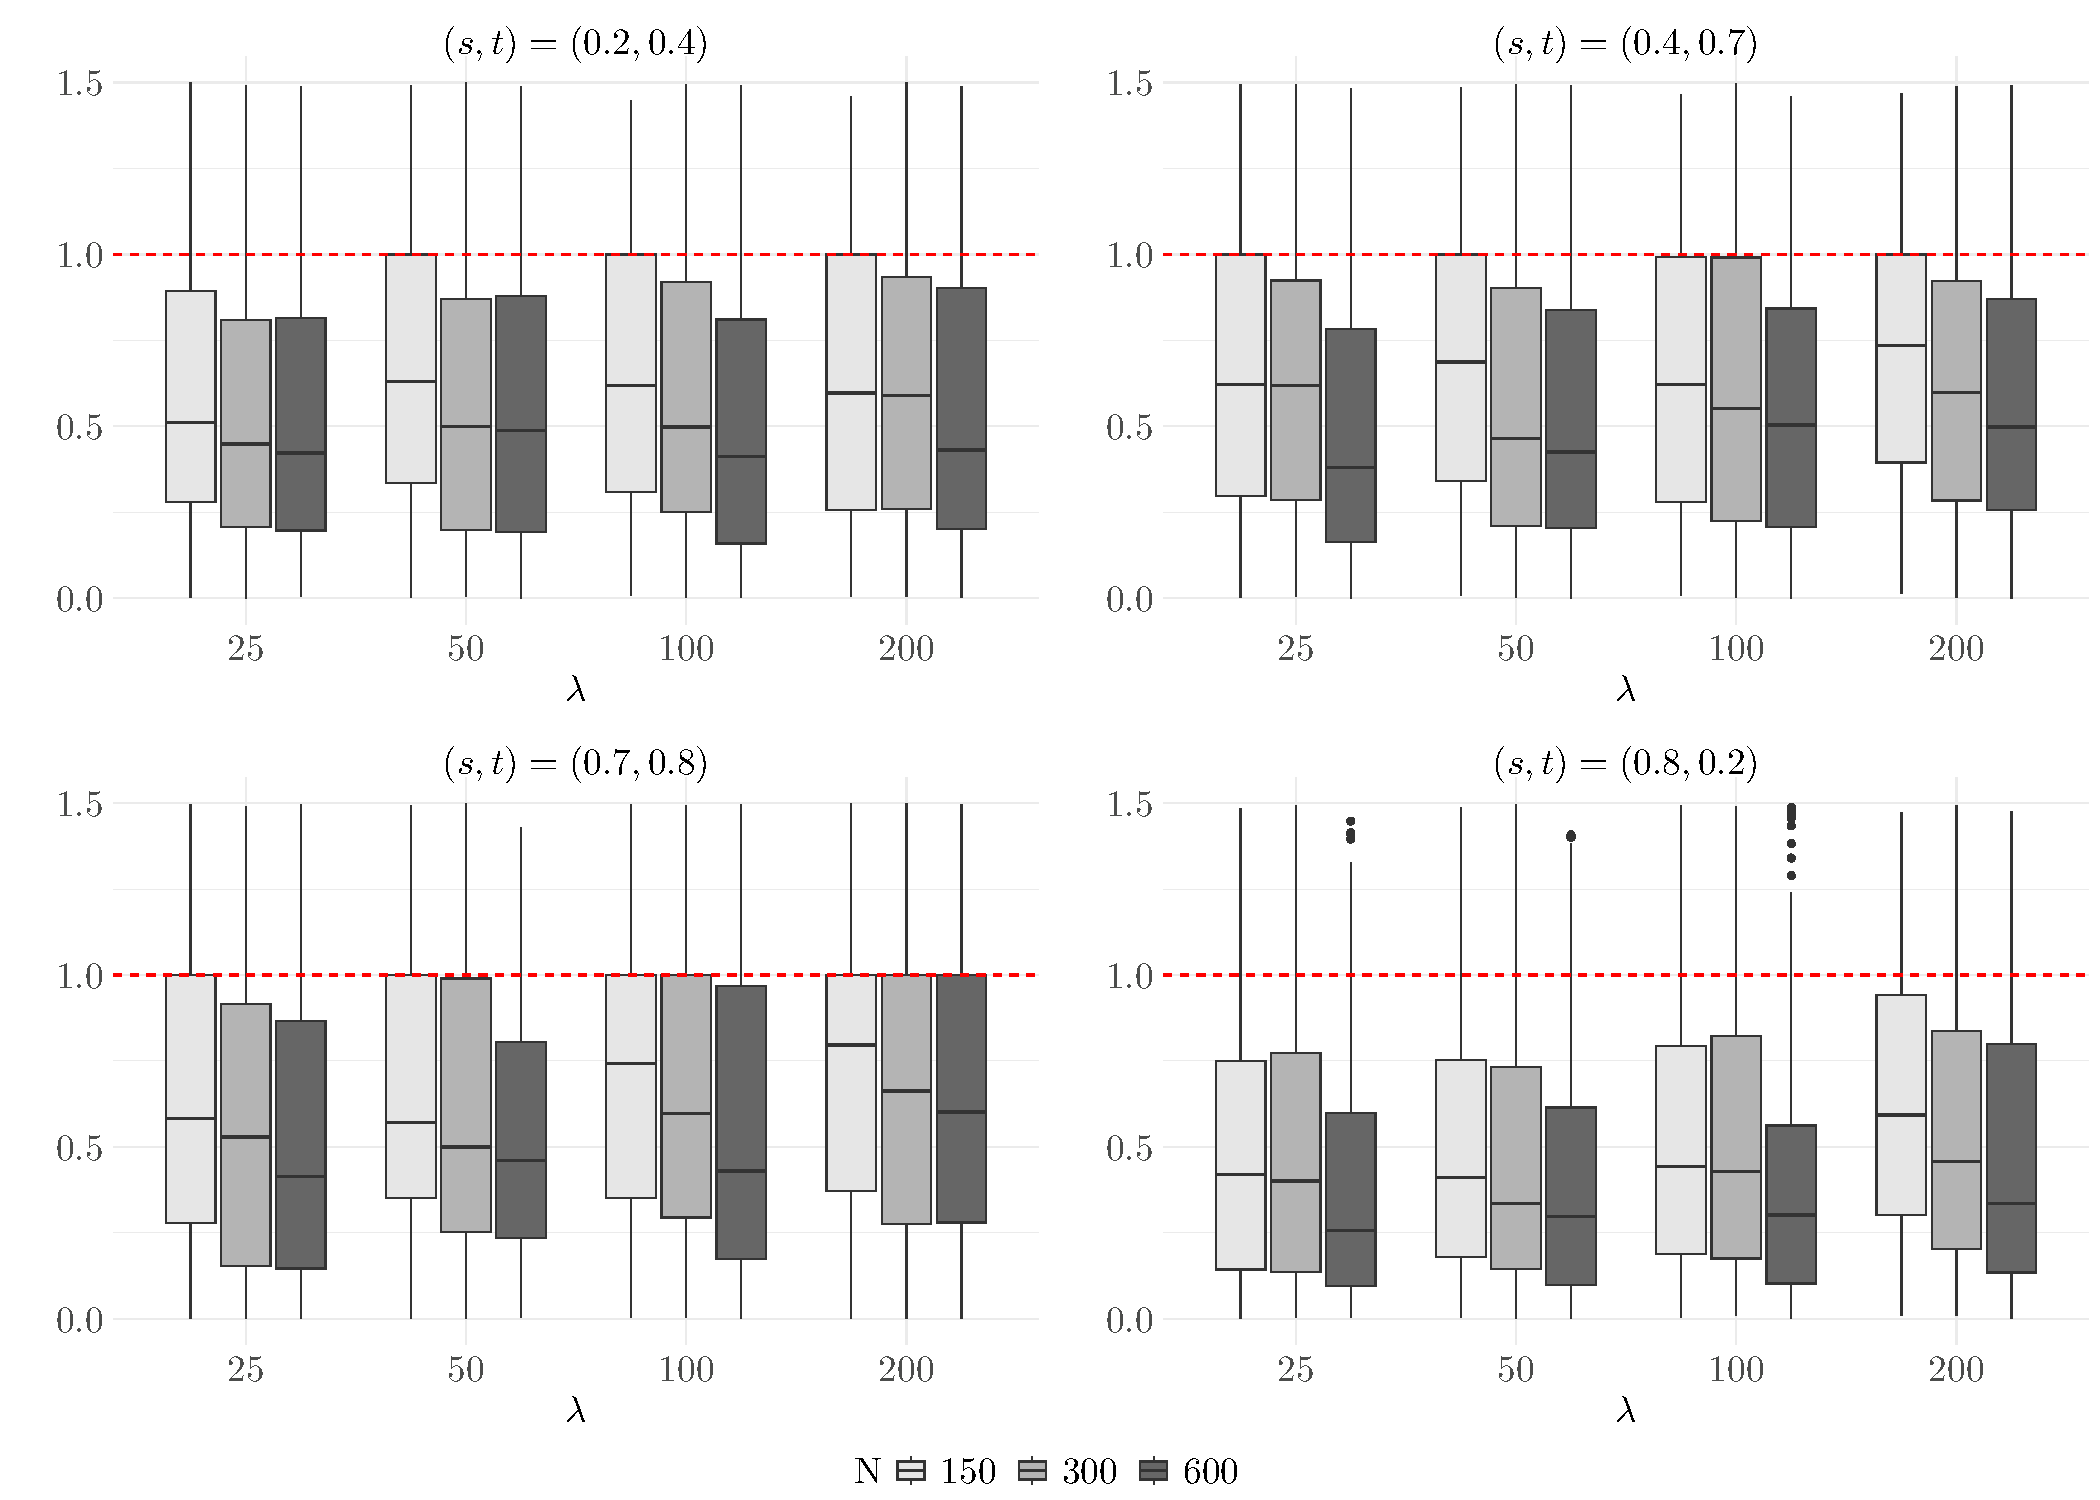
\includegraphics[width=\textwidth]{./figures/autocov/boxplot_conso_autocov_ratio_lag=1_first_4locations.pdf}
	\caption{\small \color{magenta}Boxplots of the error ratio \eqref{eq:error_ratio_autocov} of the adaptive lag-$1$ autocovariance estimator against the \texttt{MPV25} estimator, over $400$ independent functional time series generated according to \eqref{blup:FTS_mod1}. \textbf{Top left:} $(s,t) = (0.2, 0.4)$. \textbf{Top right:} $(0.4, 0.7)$. \textbf{Bottom left:} $(0.7, 0.8)$. \textbf{Bottom right:} $(0.8, 0.2)$. Within each panel the boxes are grouped along the horizontal axis by $\lambda$ and shaded by $N$, the darker the shade the larger $N$; the dashed line marks the value $1$, at which the two estimators are equally far from the benchmark. The vertical axis stops at $1.5$ and the ratios above it are not drawn.\color{black}}
	\label{fig:autocov_ratio_lag1}
\end{figure}

\color{magenta}
At lag $0$ the comparison is the same one. The single-bandwidth covariance estimator is the \texttt{MPV25} estimator at $\ell = 0$, so \eqref{eq:error_ratio_autocov} applies unchanged, with the benchmark ${\widehat{c}}_{N', 0}$ formed on the same infeasible sample. The four pairs $(s,t)$ are those of Figure~\ref{fig:autocov_ratio_lag1}, so that the two lags are read at the same points of the domain.

Figure~\ref{fig:cov_ratio_lag0} shows the boxplots of that ratio. The adaptive estimator is again the closer of the two to the benchmark, its median lying below one in $35$ of the $48$ pairs of location and setup, exactly one in $11$ and above one in $2$. The margin is nonetheless narrower than at lag $1$: the smallest median over the twelve setups is $0.628$, against $0.433$ at lag $1$.

The margin also stops tracking the distance between the exponents. The four ranges of the median overlap: $0.737$ to $1$ at $(0.7, 0.8)$, $0.628$ to $1$ at $(0.2, 0.4)$, $0.756$ to $1.052$ at $(0.4, 0.7)$ and $0.681$ to $1.063$ at $(0.8, 0.2)$, so no pair is the best throughout. This is likely due to the wider bandwidths the lag-$0$ risk selects: at three of the four pairs at least one of the two optima is larger than its lag-$1$ counterpart, so both estimators average over more of the domain and the difference between them has less room in which to show. The bandwidths themselves do order with $|H_s - H_t|$ at lag $0$, as the risk surfaces presented in the Supporting Information show; that ordering is not inherited by the accuracy.

The unit medians are more frequent here, and their origin is the one given at lag $1$: the adaptive rule selects a common bandwidth in between $6$ and $51$ of the $400$ replications of a setup at $(0.7, 0.8)$, the most of the four pairs in every setup. The truncation of the display is also the same: the estimator returns no value in $471$ of the $19200$ combinations, and $6027$ of the remaining $18729$ ratios lie at or above the axis limit of $1.5$.
\color{black}

\begin{figure}[h!]
	\centering
	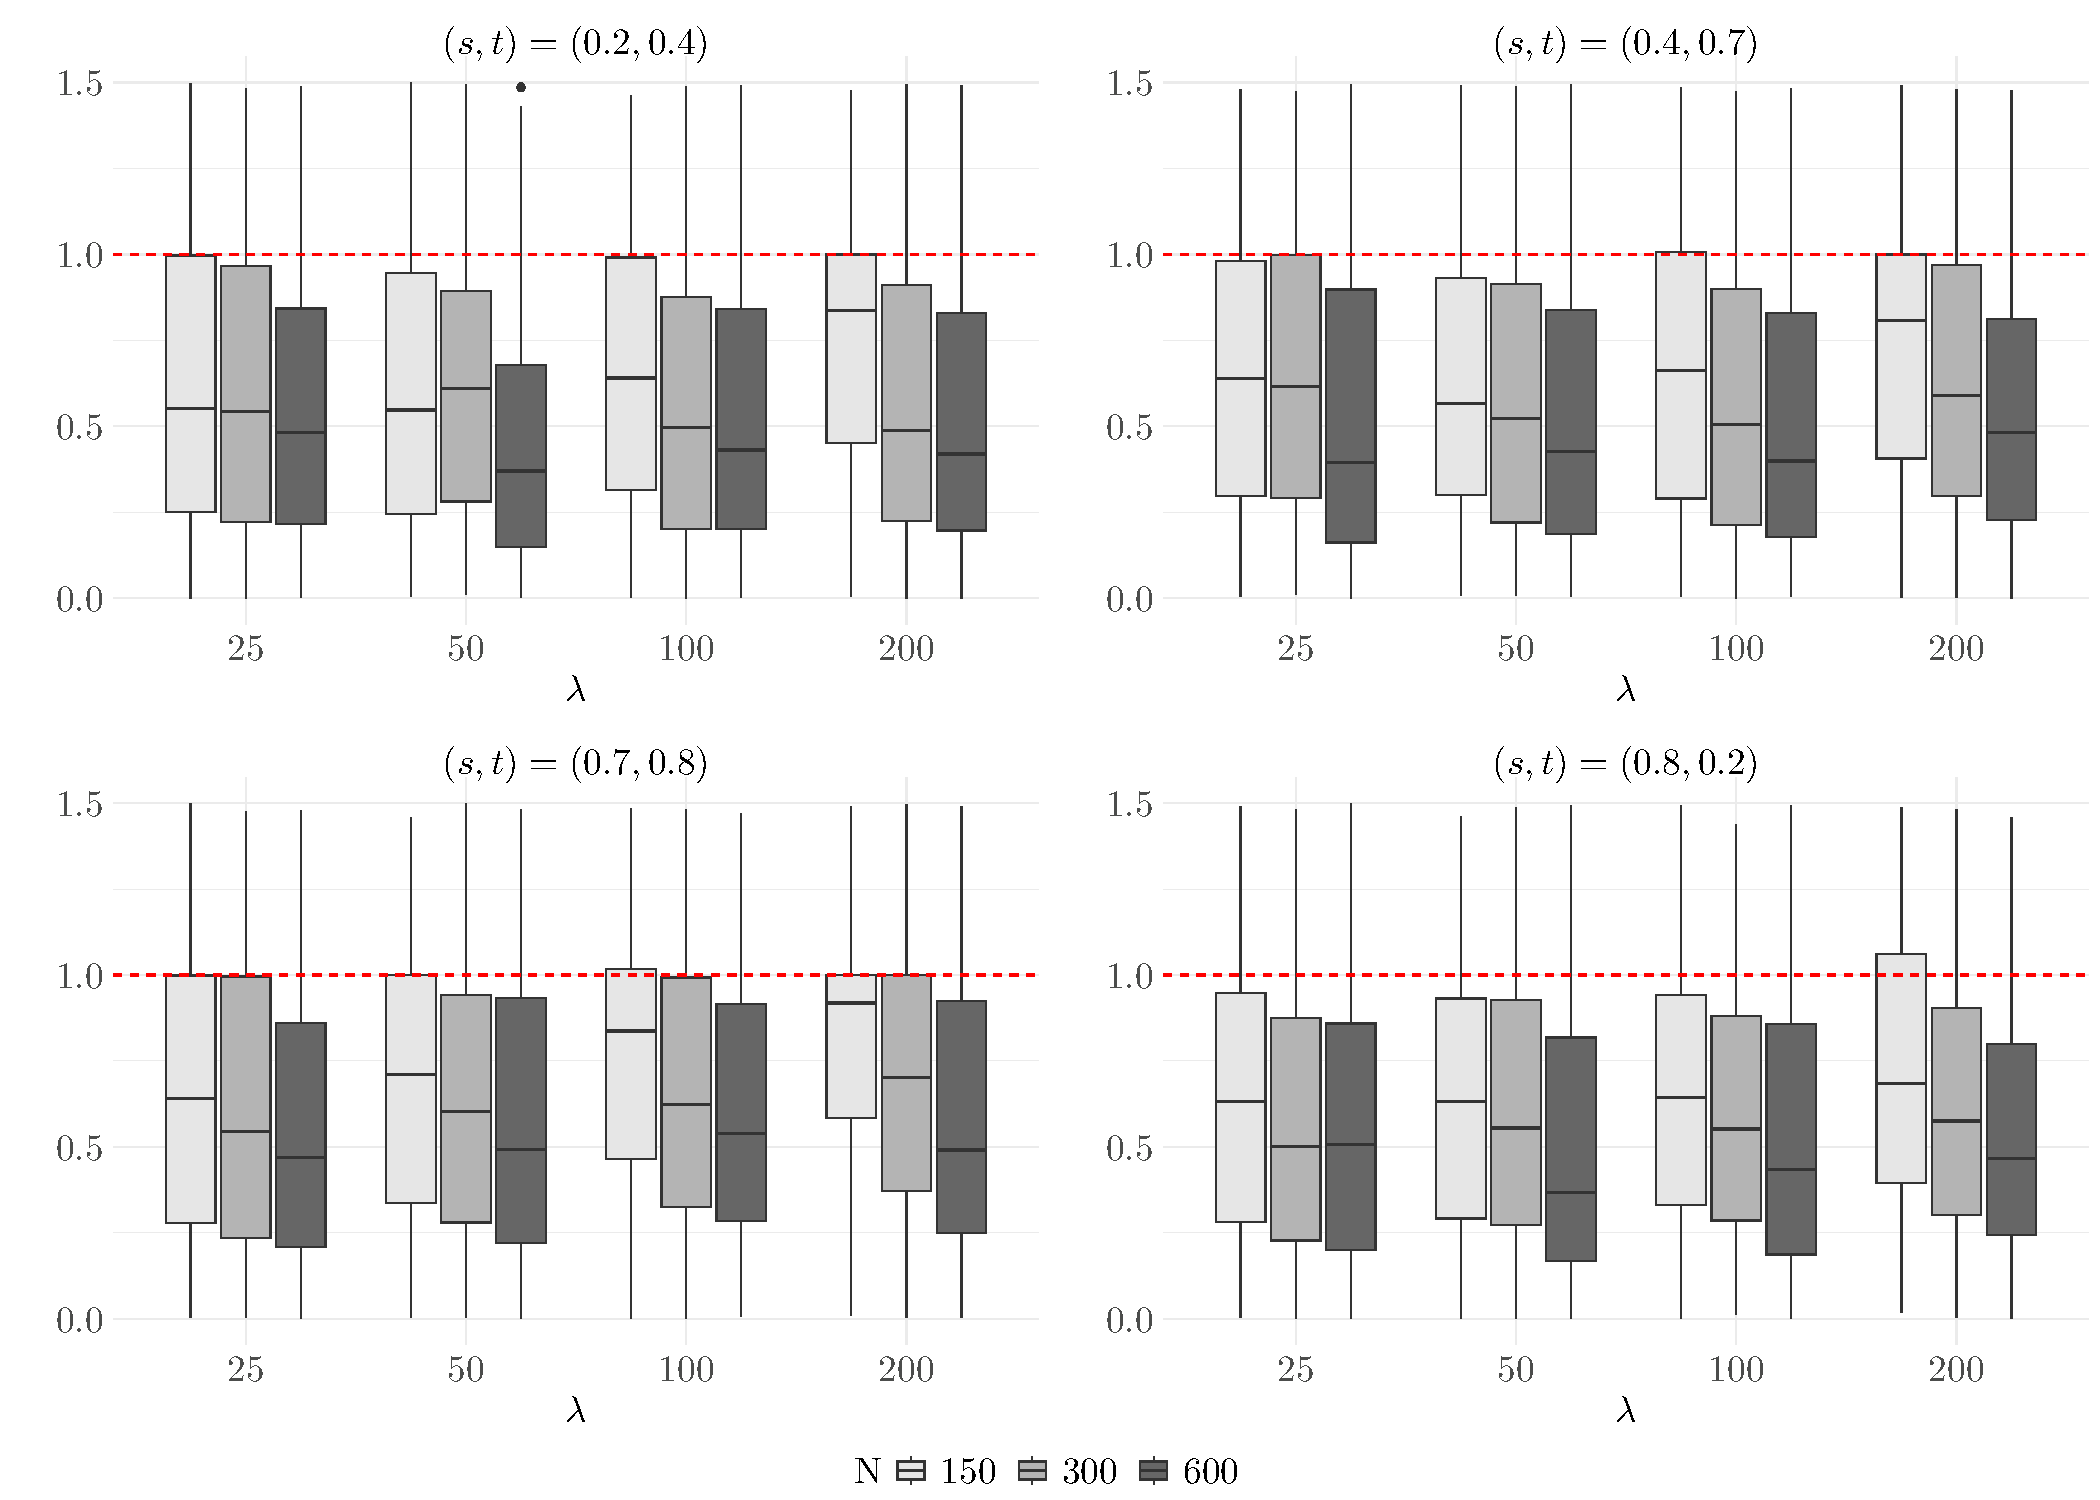
\includegraphics[width=\textwidth]{./figures/cov/boxplot_conso_cov_ratio_lag=0_first_4locations.pdf}
	\caption{\small \color{magenta}Boxplots of the error ratio \eqref{eq:error_ratio_autocov} at $\ell = 0$, of the adaptive covariance estimator against the \texttt{MPV25} estimator, over $400$ independent functional time series generated according to \eqref{blup:FTS_mod1}. \textbf{Top left:} $(s,t) = (0.2, 0.4)$. \textbf{Top right:} $(0.4, 0.7)$. \textbf{Bottom left:} $(0.7, 0.8)$. \textbf{Bottom right:} $(0.8, 0.2)$. The panels, the grouping by $\lambda$, the shading by $N$, the dashed line at $1$ and the truncation of the vertical axis are those of Figure~\ref{fig:autocov_ratio_lag1}.\color{black}}
	\label{fig:cov_ratio_lag0}
\end{figure}

\subsection{Adaptive curve prediction}\label{sec:num:prediction}

\color{magenta}
The predictor under study is the Tikhonov-regularised predictor $\mathfrak{X}^{(M_{n_0})}_{n_0+1}(t;\alpha,\sigma^2\Dd_{n_0})$ of \eqref{our_reg_blup}, with the unknown $\mu$, $c_0$, $c_1$ and $\sigma^2$ replaced by the adaptive estimators of Section~\ref{sec:emp_study:autocov}. We write $\widehat{\Xf}^{(M_{n_0})}_{n_0+1}(t;\alpha,\widehat\sigma^2\Dd_{n_0})$ for the resulting plug-in predictor, and $\alpha$ denotes throughout the Tikhonov regularisation parameter of \eqref{formula_tik_th}. The design weights $\varrho_{n_0,i}$ collected in $\Dd_{n_0}$ are those of \eqref{def_Qn}, specialised in Proposition~\ref{prop:tikhonov} to $M_{n_0}^{-1}$ under the equidistant common design and to $\{M_{n_0}\widehat g_{n_0,i}(T_{n_0,i})\}^{-1}$ under the independent design, with $\widehat g_{n_0,i}$ the leave-one-out Parzen--Rosenblatt estimator of \eqref{PR_weights}.
[TBC: the plug-in predictor is displayed but unlabelled in best\_predictor\_aout24.tex:371--373; it needs a label there so this sentence can \texttt{\textbackslash eqref} it instead of naming it]
\color{black}

\subsubsection{\color{magenta}Simulation protocol\color{black}}

\color{magenta}
Each replication draws a complete functional time series. We generate $R = 400$ independent series for each of the twelve setups $(N, \lambda) \in \{150, 300, 600\} \times \{25, 50, 100, 200\}$, and within a series we predict the last curve from the one preceding it. The estimates entering the predictor are computed on the curves before the target, so that no information about the curve being predicted enters its own prediction.

A series is generated from the autoregressive model \eqref{blup:FTS_mod1}. The innovations are multifractional Brownian motions with the local Hölder exponent $H_t = 0.4 + 0.4\,t$, which rises across the domain from $0.4$ to $0.8$, and with Hölder constant $0.1$. Each innovation carries a centred Gaussian intercept of its own, of standard deviation $0.0224$, drawn once per curve. Without it every curve leaves the origin at the same point, the multifractional Brownian motion being pinned at zero there. The operator norm of $\psi$ is set to $0.5$, and a burn-in of $100$ curves is discarded.

Each series carries both designs on the same curves. Under the independent design the number of points per curve is drawn uniformly on the integers between $0.8\lambda$ and $1.2\lambda$, and the design points are independent draws from the uniform distribution on $(0,1]$; under the common design every curve is observed on the shared equidistant grid of $\lambda$ points. Both are observed with the same centred Gaussian noise of standard deviation $0.007$, and the noiseless curve is retained alongside. Running the study on each design in turn therefore isolates the effect of the design, everything else being held fixed.

Every parameter is selected inside the replication, on that replication's own fit sample, so that a replication carries no information from any other. The bandwidths are selected by the adaptive rules of Section~\ref{sec:emp_study:autocov}, the design-density bandwidth and the Tikhonov parameter by the cross-validation procedures described in the Supplementary Material. One seed is drawn per replication rather than per curve, since the innovations must remain successive draws from a single advancing stream; the seed depends on the replication's identity and not on its position in the loop.
\color{black}

\subsubsection{\color{magenta}Autoregressive effect\color{black}}

\color{magenta}
The adaptive predictor depends on adaptive estimates of the mean, covariance and lag-$1$ autocovariance functions. To describe the strength of dependence between the target curve and the curve preceding it, we compute a functional analogue of the autocorrelation function for real-valued time series. The Functional Autocorrelation Function (FACF) at lag~$\ell$, considered by \citet{horovath_2016}, is defined as
\color{black}
\begin{equation}\label{eq:blup:facf}
	\color{magenta}\widehat{\rho}_\ell =
	\|\widehat{c}_{N,\ell}\|\left[\int \widehat{c}_{N,0}(t,t)dt\right]^{-1},\color{black}
\end{equation}
\color{magenta}
where $\widehat{c}_{N,\ell}$ estimates $c_\ell$, and $\|\cdot\|$ denotes the standard norm in $\LL^2_\Hh$. Moreover, $0 \leq \widehat{\rho}_\ell \leq 1$. The FACF also serves as an empirical check for the presence of an autoregressive effect in the FTS. In fact, if there were no autoregressive effect, then $c_1$ would vanish, the operator $\Pi_{n_0,1}^\star$ of \eqref{our_reg_blup} would be null, and the predictor would reduce to the mean function $\mu$, the lagged curve contributing nothing.\color{black}

\subsubsection{\color{magenta}Weighted integrated squared error\color{black}}

\color{magenta}
The curve to be predicted is observed at its own design points $T_{n_0+1,i}$, $1\leq i \leq M_{n_0+1}$, and the predictor is scored there. Let $\varrho_{n_0+1,i}$ be the design weights of \eqref{def_Qn} formed on that curve, that is $M_{n_0+1}^{-1}$ under the equidistant common design and $\{M_{n_0+1}\widehat g_{n_0+1,i}(T_{n_0+1,i})\}^{-1}$ under the independent design. The weighted integrated squared error of the adaptive predictor is
\color{black}
\begin{equation}\label{eq:weighted_ise}
	\color{magenta}\mathrm{ISE}\big(\widehat{\Xf}^{(M_{n_0})}_{n_0+1}\big) = \sum_{i=1}^{M_{n_0+1}} \varrho_{n_0+1,i}\left\{Y_{n_0+1,i} - \widehat{\Xf}^{(M_{n_0})}_{n_0+1}\big(T_{n_0+1,i};\alpha,\widehat\sigma^2 \Dd_{n_0}\big)\right\}^2,\color{black}
\end{equation}
\color{magenta}
a discrete Riemann sum against the measure $Q_{n_0+1}$ of \eqref{def_Qn}, which weights each design point by the inverse of the local design density and so does not over-count regions where observations happen to concentrate. Replacing $Y_{n_0+1,i}$ by the noiseless $X_{n_0+1}(T_{n_0+1,i})$ gives a second variant; the two differ by the measurement-error variance, an additive offset that does not cancel in a ratio.

The same functional is the criterion by which $\alpha$ is selected: the cross-validation score of the Tikhonov selection is \eqref{eq:weighted_ise} evaluated on held-out curves. Definition, scoring and selection are therefore one object, not three.

The quantity in \eqref{eq:weighted_ise} is one number per replication, so it is reported as a distribution over the $R = 400$ replications rather than as a pointwise curve. For each setup $(N,\lambda)$ and each design we report its mean, median and standard deviation, in both variants, and we display the distribution of its logarithm as boxplots grouped by $\lambda$. Replications on which the score is not finite are dropped, and their number is reported alongside. A decomposition into bias and variance is not available under the independent design, where each replication draws its own design points and there is no shared location at which the predictions could be averaged.
[TBC: \eqref{eq:weighted_ise} is written here because best\_predictor\_aout24.tex defines no ISE, weighted or otherwise. Two points need ratification there. First, \eqref{def_Qn} requires $\sum_i \varrho_{n,i} = 1$, which the independent-design form $\{M_n \widehat g_{n,i}\}^{-1}$ of Proposition~\ref{prop:tikhonov} satisfies only in the limit; 22\_simulation\_blup.R:143--144 renormalises it exactly, so the paper and the implementation disagree on a constant. Second, the authority defines $\varrho$ and $\Dd$ on the conditioning curve $n_0$ only, whereas the score above needs them on the target curve $n_0+1$]
\color{black}

\color{magenta}
[TBC: results for \eqref{eq:weighted_ise}, both designs. Requires 22\_simulation\_blup.R then 32\_figures\_blup.R; data-simulation/estimates/ has no blup/ directory and figures/blup/ is empty. The replacement for the superseded bias/standard-deviation table is a five-decimal table of Mean, Median and Sd for each of the two variants of \eqref{eq:weighted_ise}, written by 32\_figures\_blup.R:55--80. A bias/variance split is not available: under the random design each replication draws its own grid. Any comment on how the ISE varies with $t$ must be dropped rather than carried over --- \eqref{eq:weighted_ise} is a single number per replication, not a pointwise curve]
\color{black}

\subsubsection{\color{magenta}Comparison under the independent design\color{black}}

\color{magenta}
Under the independent design we compare our predictor with the procedure of \citet{rubin2020sparsely}, referred to as \texttt{RP20}. That procedure is also based on the best linear unbiased predictor: the mean is estimated by a local linear smoother, the lag-$\ell$ autocovariance by a local linear surface smoother away from the diagonal and by a local quadratic smoother on it, and the smoothing bandwidths are selected by $K$-fold cross-validation coupled with Bayesian optimisation. A single bandwidth is selected for the whole domain, whereas ours varies with the location.

The comparison is confined to the independent design because \texttt{RP20} is constructed for sparsely and irregularly sampled curves, which is the regime the common grid removes.

The competitor is fitted on exactly the data our predictor is fitted on. For each replication we export the noisy observations of the curves preceding the target, together with the target curve at its own design points, in the form the implementation consumes; one file is written per replication. Both predictors are then fitted on that estimation sample and evaluated for the same target curve.

The two are scored on the evaluation points they share. \texttt{RP20} returns its prediction on a fixed grid while ours is evaluated at the target curve's own design points, so each design point is carried to its nearest grid point and the squared error of each predictor is integrated by the trapezoidal rule against the noiseless target curve. This score is not \eqref{eq:weighted_ise}: it is unweighted, and it is taken against a common evaluation set rather than against the design measure of the target curve. We refer to it as the trapezoidal error, and we compare the two predictors through the logarithm of its ratio, a value below zero indicating the smaller error for the adaptive predictor. The design weights of \eqref{eq:weighted_ise} would in any case cancel from such a ratio.
[TBC: the evaluation grid \texttt{RP20} returns is described in the superseded text as a regular grid of $241$ points with a B-spline projection used to reduce the cost of the Bayesian optimisation. Neither number nor the projection is attested in any current file, so both are omitted here; restate them from the MATLAB implementation once it has been run]

[TBC: results. Requires the \texttt{RP20} outputs, which 32\_figures\_blup.R:130--134 reads from data-simulation/estimates/RP20/; that directory does not exist. The figure is a boxplot of the log trapezoidal-error ratio, grouped by $\lambda$ and shaded by $N$, with a dashed line at zero]
\color{black}

\subsubsection{\color{magenta}Comparison under the common design\color{black}}

\color{magenta}
Under the common design we compare our predictor with the procedure of \citet{zhao2026functional}, referred to as \texttt{Z26}. That procedure estimates the autoregressive operator by a single Tikhonov regularisation,
\color{black}
\begin{equation}\label{eq:zhao_estimator}
	\color{magenta}\widehat{\psi}(\cdot\,;\alpha_N) = \widehat{C}_1 \left(\widehat{C}_0 + \alpha_N \mathrm{Id}\right)^{-1},\color{black}
\end{equation}
\color{magenta}
with $\alpha_N \to 0$, and predicts the next curve by $\widehat\mu + \widehat\psi(X_{n_0} - \widehat\mu)$. It dispenses with the projection onto the leading eigenfunctions of $C_0$ that a truncation-based estimator requires, so a single regularisation parameter is selected rather than two. The parameter is selected by cross-validation, as ours is, which makes the two procedures comparable on the choice of regularisation and not only on the prediction.

The comparison is confined to the common design because \eqref{eq:zhao_estimator} is defined for curves observed on a shared grid: the empirical operators $\widehat{C}_0$ and $\widehat{C}_1$ are then formed as $\lambda \times \lambda$ matrices from the discretised curves, without any preliminary smoothing. Under the independent design no two curves share their design points, and the operators would have to be built from smoothed curves, which would compare our smoothing with itself rather than the two predictors.

Both procedures are fitted on the curves preceding the target and predict the same target curve. Since both are evaluated on the shared grid, no interpolation is needed and the two are scored by \eqref{eq:weighted_ise} itself, whose weights reduce to $\lambda^{-1}$ there. We compare them through the logarithm of the ratio of their scores.
[TBC: \eqref{eq:zhao_estimator} and the assumptions attached to it are restated from best\_predictor\_aout24.tex:129--143 and 399--403, which summarise \citet{zhao2026functional}. Verify against the paper itself before submission, and settle whether $\widehat\mu$ is the adaptive mean estimator or the empirical mean of the gridded curves]

[TBC: results. No implementation exists --- \texttt{Z26} appears in no script of the numerical study, so the estimator, its cross-validation and the export have still to be written]
\color{black}

\subsection{Real data applications}\label{sec:num:realdata}

\color{magenta}
[TBC: shared opening paragraph stating that the two applications are chosen to exercise the two designs the method covers]
\color{black}

\subsubsection{\color{magenta}NOTPERP intraday log-return curves\color{black}}

\color{magenta}
[TBC: random-design application. Descriptive material is reusable from paper\_for\_reference/NOTPERP\_descriptive\_analysis/report/NOTPERP\_data.tex --- the ByBit provenance, the observation-time map $T_{n,i} = (\tau_{n,i} - a_n)/86400$, the cumulative intraday log-return, the cleaned sample size and the local regularity range --- but its numbers come from 01\_NOTPERP\_analysis.R and must be re-verified against 41\_notperp\_download\_clean.R. Prediction results are unavailable: data-NOTPERP/estimates/ is empty and 42\_app\_notperp.R does not run to completion, see adaptiveFTS-issues.md]
\color{black}

\subsubsection{\color{magenta}French electricity curves\color{black}}

\color{magenta}
[TBC: common-design application. Provenance reusable from Numerical\_analysis-2025-06-v1.tex:244 --- ODR\'E, 122 consumption curves at 96 quarter-hourly points, 122 photovoltaic curves restricted to 61 points over 04:00--19:00, 152 hydroelectric curves at 96 points, all normalised by the maximum. 40\_app\_energy.R:26--28 additionally steps the target curve back by 10 for photovoltaic and 12 for hydroelectric because their last curves are incomplete. data-energy/estimates/ predates the current script and must be re-run before any number is quoted]
\color{black}
